\chapter{Mixed-Bag Solver Overview}\label{chap:mixedBagSolver}

When humans solve jigsaw puzzles, it is common that they first correctly assemble small regions of the puzzle and then merge those smaller regions to form larger regions.  The Mixed-Bag Solver presented in this thesis is based off this solving strategy.  The solver consists of five distinct stages, namely: segmentation, stitching, hierarchical clustering of segments, seed piece selection, and final assembly.  The flow of the algorithm is shown in Figure~\ref{fig:multipuzzleSolverArchitecture}.  The pseudocode for the solver, including the input(s) and output of each stage is shown in Algorithm~\ref{alg:mixedBagSolver}. 

The following subsections describe each of the Mixed-Bag Solver's stages/subfunctions.  An additional associated component referred to as the ``assembler'' (not shown in Figure~\ref{fig:multipuzzleSolverArchitecture}) is also discussed.

\begin{figure}[ht!]
	\centering
		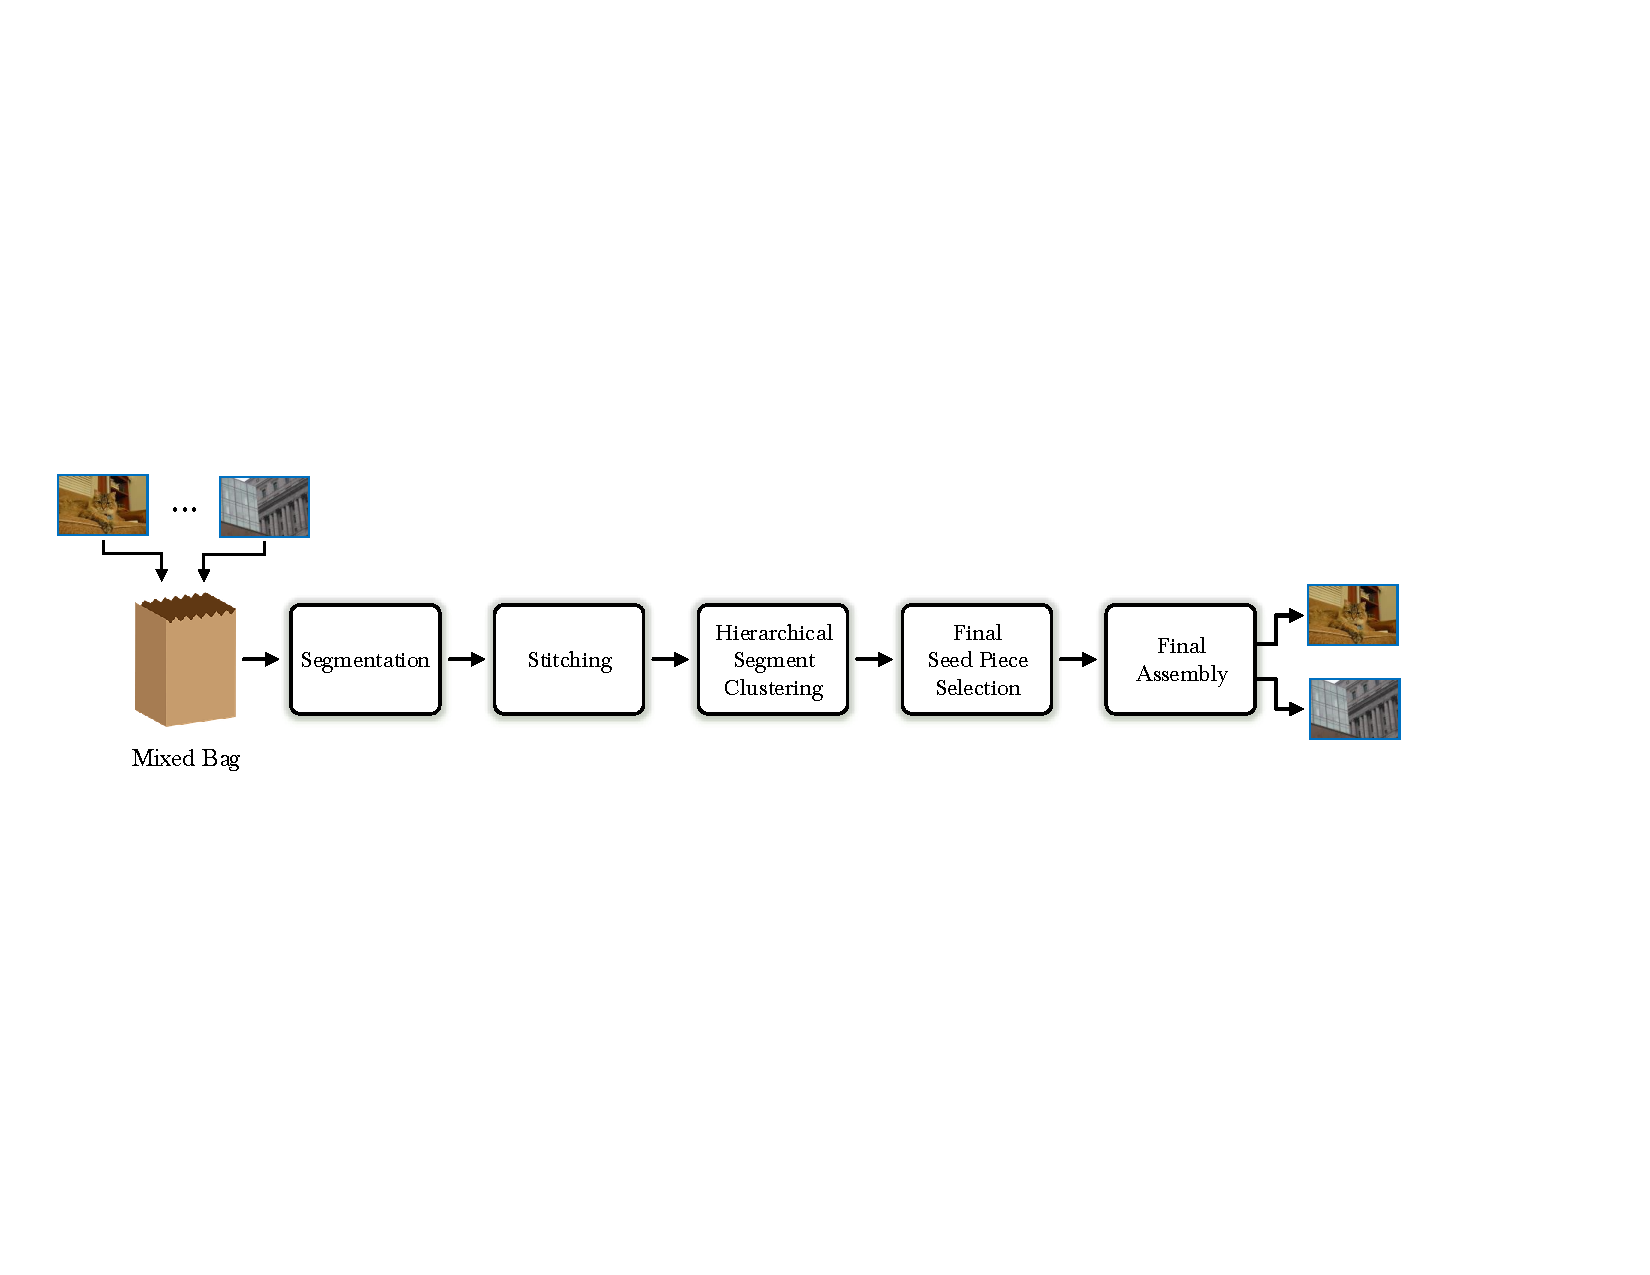
\includegraphics[width=1.0\textwidth]{images/cropped_algorithm_structure_overview.pdf}
	\caption{Relationship between the Mixed-Bag Solver's Components}\label{fig:multipuzzleSolverArchitecture}
\end{figure}

\begin{algorithm}[tb]
\caption{Pseudocode for the Mixed-Bag Solver}\label{alg:mixedBagSolver}
\begin{algorithmic}[1]
\Function{MixedBagSolver}{$puzzle\hspace{-0.8pt}\_pieces$}
    \State $saved\_segments \gets \textproc{Segmentation}\text{(} puzzle\hspace{-0.8pt}\_pieces \text{)}$
	\State $overlap\_matrix \gets \textproc{Stitching}\text{(} saved\_segments \text{, } puzzle\hspace{-0.8pt}\_pieces \text{)}$
	\State $clusters \gets \textproc{HierarchicalClustering} \text{(}saved\_segments \text{, } overlap\_matrix \text{)}$
	\State $seed\_pieces \gets \textproc{FindSeedPieces} \text{(} clusters \text{)}$
	\State $solved\_puzzles \gets \textproc{RunFinalAssembly} \text{(} seed\_pieces \text{, } puzzle\hspace{-0.8pt}\_pieces \text{)}$
    \State \Return $solved\_puzzles$
\EndFunction
\end{algorithmic}
\end{algorithm}

\section{Assembly}\label{sec:SolverAssembler}

The assembler places the individual pieces in the solved puzzle.  The Mixed-Bag Solver's architecture is largely independent of the particular assembler used.  Hence, any improvements or modifications made to the assembler can be directly incorporated into the Mixed-Bag Solver to improve the solver's overall performance.  What is more, if particular assemblers perform better in specific applications, the assemblers can be interchanged.  This provides the Mixed-Bag Solver with significant flexibility and upgradability to maximize performance across a wide range of applications.

This thesis uses the assembly algorithm proposed by Paikin~\& Tal~\cite{paikin2015} as it is the current state of the art and because it is one of the few assemblers that natively supports Mixed-Bag puzzles.  The following two subsections describe this thesis' implementation of their assembler as well as the time complexity of assembly.

\subsection{Assembler Implementation}\label{sec:assemblerImplementation}

Paikin~\& Tal wrote their algorithm in Java, and as of this publication, the source code has not been released.  Hence, their algorithm was fully reimplemented as part of this thesis using the description in~\cite{paikin2015}.  This thesis' implementation is written in the Python programming language and is fully open-source. While the results generated by the two algorithms should be very similar, it is expected that the underlying software architecture is significantly different. 

No execution time comparisons between Paikin~\& Tal's algorithm and the Mixed-Bag Solver are included with this thesis since Java is generally significantly faster than Python~\cite{pythonJavaComparison}.  Instead, the next subsection reviews the expected time complexity of both their algorithm and the Mixed-Bag Solver.

\subsection{Assembler Time Complexity}\label{sec:assemblerTimeComplexity}

Paikin~\& Tal's assembler relies on a set of inter-puzzle piece similarity metrics.  Similar to all other jig swap solvers, these distances are calculated between all pairs of pieces, making the time required to calculate inter-piece similarity $O(n^2)$, where $n$ is the number of puzzle pieces.  If an input image has sufficient inter-piece variation, then the time complexity to place all pieces is $\Theta(n \text{lg}(n))$, since a heap is used in this thesis' implementation to determine the piece placement order.  However, if most pieces are sufficiently similar that there are relatively few best buddies, then piece placement can be as slow as $O(n^3)$ as the inter-piece similarity may need to be recalculated after each piece is placed.

The Mixed-Bag Solver performs assembly at least once during the segmentation stage (usually more times), and placement is performed another time during the final assembly stage.  Hence, while the execution time for the Mixed-Bag solver is necessarily longer than any assembler that may be used, they both share the same time complexity since the number of times placement is performed is not directly related to the number of puzzle pieces.

\section{Segmentation}\label{sec:Segmentation}

Segmentation provides basic structure to the bag of puzzle pieces by partitioning these pieces into disjoint sets, referred to here as segments.  These segments are partial puzzle assemblies where there is a high degree of confidence that the pieces are placed correctly. As detailed in Algorithm~\ref{alg:mixedBagSolver}, the only input to the segmentation stage is the bag of puzzle pieces; the solver takes no other inputs.  It is expected that pieces from the same ground-truth input may be assigned to multiple segments.  Section~\ref{sec:hierarchicalClustering} describes how these segments are merged using hierarchical clustering.

\subsection{Overview of the Segmentation Procedure}

Algorithm~\ref{alg:segmentation} outlines the basic segmentation framework; the implementation is iterative and will have one or more rounds.  In each round, all pieces not yet assigned to a saved segment are assembled as if they all belong to a single ground-truth image.  This strategy eliminates the need to make any assumptions at this early stage regarding the number of input puzzles. 

Section~\ref{sec:segmentPuzzle} describes the procedure used to create the individual segments. The largest segment in each round is passed to the Stitching stage described in Section~\ref{sec:stitching}.\footnote{All saved segments must exceed a minimum size.  For this thesis, it was observed that a minimum segment size of 7 provided the best balance between solution quality and algorithm execution time.} Similarly, the multiplicative scalar term ``\textit{$\alpha$}'' in Algorithm~\ref{alg:segmentation} dictates which other segments are also passed to the Stitching stage.  In this thesis, \textit{$\alpha$} was set to~0.5, meaning that all segments that were at least half the size of the largest segment were also saved.  This approach provided sufficient balance between finding the largest possible segments while limiting overall execution time.

Once a piece is assigned to a saved segment, it is removed from the set of unassigned pieces.  Hence, those pieces will not be placed in future segmentation rounds.  Segmentation continues until all pieces have been assigned to sufficiently large segments or no segment exceeds the minimum allowed segment size.

\begin{algorithm}[tb]
\caption{Pseudocode for the Complete Segmentation Algorithm}\label{alg:segmentation}
\begin{algorithmic}[1]
\Function{Segmentation}{$puzzle\hspace{-0.8pt}\_pieces$}
    \State $saved\_segments \gets \{ \}$
    \State $unassigned\_pieces \gets \{ puzzle\hspace{-0.8pt}\_pieces \}$
    \Loop
        \State $solved\_puzzle \gets \textproc{RunSinglePuzzleAssembly}(unassigned\_pieces)$
        \State $puzzle\hspace{-0.8pt}\_segments \gets \textproc{SegmentPuzzle}(solved\_puzzle)$
        \State $max\_segment\_size \gets \text{maximum size of segment in } puzzle\hspace{-0.8pt}\_segments$
        \If{$max\_segment\_size \text{ < } smallest\_allowed$}
			\State \Return $saved\_segments$
        \EndIf
        \ForEach{$segment \in puzzle\hspace{-0.8pt}\_segments$}
            \If{$|segment| \text{ > } \text{max}(\alpha {} \cdot {} max\_segment\_size, \text{ } smallest\_allowed)$}
                \State $\text{add } segment \text{ to } saved\_segments$
                \State $\text{remove pieces in } segment \text{ from } unassigned\_pieces$
            \EndIf
        \EndFor
	\EndLoop
\EndFunction
\end{algorithmic}
\end{algorithm}

\subsection{Partitioning a Puzzle into Segments}\label{sec:segmentPuzzle}

The function ``\textproc{SegmentPuzzle}'' in Algorithm~\ref{alg:segmentPuzzle} partitions a solved puzzle into disjoints segments.  The procedure is adapted from the region growing segmentation algorithm proposed by Pomeranz~\textit{et al.}, where it was shown to have greater than 99.7\% accuracy identifying genuine neighbors~\cite{pomeranz2011}. 

\begin{algorithm}[tb]
\caption{Pseudocode for Segmenting a Solved Puzzle}\label{alg:segmentPuzzle}
\begin{algorithmic}[1]
\Function{SegmentPuzzle}{$solved\_puzzle$}
    \State $puzzle\hspace{-0.8pt}\_segments \gets \{ \}$
    \State $unassigned\_pieces \gets \{ \text{all pieces in } solved\_puzzle \}$
    \While{$|unassigned\_pieces| \text{ > } 0$}
        \State $segment \gets \text{ new empty segment}$
        \State $seed\_piece \gets \text{next piece in } unassigned\_pieces$
        \State $queue \gets [seed\_piece]$
        \While{$|queue| \text{ > } 0$}
            \State $piece \gets \text{next piece in } queue$
            \State $\text{add } piece \text{ to } segment$
            \ForEach{$neighbor \text{ of } piece$}
            	\If{$\textproc{IsBestBuddies}(neighbor, piece)$}
            		\State $\text{add } neighbor \text{ to } queue$
            		\State $\text{remove } neighbor\_piece \text{ from } unassigned\_pieces$
            	\EndIf
            \EndFor
        \EndWhile
        \State $articulation\_points \gets \textproc{FindArticulationPoints}(segment)$
        \State $\text{remove } articulation\_points \text{ from } \textit{segment}$
		\State $disconnected\_pieces \gets \textproc{FindDisconnectedPieces}(segment)$ 
		\State $\text{remove } disconnected\_points \text{ from } segment$
        \State $\text{add } \textit{articulation\_points} \text{ and } \textit{disconnected\_pieces} \text{ to } \textit{unassigned\_pieces}$               	
		\State $\text{add } segment \text{ to } puzzle\hspace{-0.8pt}\_segments$	
    \EndWhile
    \State \Return $puzzle\hspace{-0.8pt}\_segments$
\EndFunction
\end{algorithmic}
\end{algorithm}

Whenever a piece, including the seed, is added to a segment, the algorithm examines all of that piece's neighbors.  These adjacent pieces are also added to the segment if they are in the pool of unassigned pieces and if their neighbor inside the segment is a ``best buddy'' (as checked by the predicate ``\textproc{IsBestBuddies}'' in Algorithm~\ref{alg:segmentPuzzle}).  The growth of a segment terminates when there are no neighboring pieces that satisfy these two criteria. 

In Pomeranz \textit{et al.}'s segmentation algorithm, no changes were made to a segment after it reached its maximum size.  Their approach is sufficient when solving only a single puzzle at a time.  However, in Mixed-Bag puzzles, it is common that correctly assembled regions from different ground-truth inputs are joined into a single segment; this is usually through a very tenuous linking in the form of narrow bridges no wider than a single piece.  Section~\ref{sec:articulationPoints} describes how the Mixed-Bag Solver post-processes each segment to prevent this erroneous segment merging.

\subsection{Articulation Points}\label{sec:articulationPoints}

A segment can be modeled as a graph with a single connected component.  The individual puzzle pieces represent the vertices while the edges are the best buddy relationships between adjacent pieces.  An articulation point is any vertex (i.e., puzzle piece) in the graph whose removal increases the number of connected components.  The Mixed-Bag Solver identifies the articulation points using the algorithm proposed by~\cite{cormenIntroToAlgorithms}; these articulation pieces are then removed from the segment and returned to the set of unassigned pieces.  This step necessarily causes some other pieces to become disconnected from the segment's seed.  These disconnected pieces are also removed from the segment and marked as unassigned. Once this has been completed, the segment is in its final form.

\subsection{Segmentation Example}

Appendix~\ref{app:segmentedOutput} shows an example of a single round of segmentation with two images as the input. This is included to provide a visual reference of the segmentation process.

\section{Stitching}\label{sec:stitching}

As discussed previously, a segment represents an ordering of pieces where there is a particularly high degree of confidence that the placement is correct.  In areas of an image with little inter-piece variation, the segmenter may not have high confidence that the puzzle is assembled correctly.  This often leads to a single ground-truth image being partitioned into multiple segments. Since the Mixed-Bag Solver is not supplied with the number of input images, it must quantify the extent to which any pairs of segments are related to ensure it can accurately estimate the number of ground-truth inputs.  

It is expected that two segments that were adjacent in a ground-truth image would eventually merge if one segment were allowed to expand. Since it is not known in which relative direction the adjacent segment may be located, the segment should be allowed to grow in all directions; however, the segment should not be forced to expand in a certain direction as it may lead to the formation of erroneous inter-segment coupling.  This concept is the foundation of the inter-segment stitching used by the Mixed-Bag Solver.  This stitching process is described in the following subsections.

\subsection{Mini-Assemblies and Stitching Pieces}

As mentioned previously, a segment should be allowed, but not forced, to expand in all directions in order to identify related segments.  To achieve this, the Mixed-Bag Solver introduces the concept of a ``mini-assembly,'' which is similar to the standard assembly process described in Section~\ref{sec:SolverAssembler}, with the expectation that only a limited number of pieces are placed.\footnote{In this thesis, a mini-assembly places exactly 100 pieces.}  The seeds for each of these mini-assemblies is referred to as a ``stitching piece'' since they serve the role of ``stitching'' together associated segments.

\subsection{Selecting the Stitching Pieces}\label{sec:stitchingPieceSelection}

If stitching pieces are poorly selected, two divergent, yet deleterious outcomes may occur.  First, placing the stitching pieces too close to one another can add significant overhead without creating much tangible value.  In contrast, if the stitching pieces are too far apart, the solver may not be able to detect subtle inter-segment relationships.  Algorithm~\ref{alg:selectStitchingPieces} details the procedure used by the Mixed-Bag Solver to select the stitching pieces that balances these two concerns.  The implementation of this algorithm is described in detail in the following two subsections.

\begin{algorithm}[tb]
\caption{Pseudocode for Selecting the Stitching Pieces in a Segment}
\label{alg:selectStitchingPieces}
\begin{algorithmic}[1]
\Procedure{FindStitchingPieces}{$segment\_pieces$}
	\State $\textproc{FindPieceDistanceToOpen}(segment\_pieces)$
	\State $segment\_stitching\_pieces \gets \{ \}$
    \State $segment\_grid\_cells \gets \textproc{PartitionIntoGrid}(segment)$
	\ForEach{$grid\_cell \in segment\_grid\_cells$}
		\If{$\textproc{HasPieceAdjacentToOpen}(grid\_cell)$}
			\State $candidates \gets \{ pieces \} \in grid\_cell \text{ closest to } target\_distance\_to\_open$
			\State $stitching\_piece \gets piece \in candidates \text{ closest to center of } grid\_cell$
			\State $\text{add } stitching\_piece \text{ to } segment\_stitching\_pieces$
		\EndIf
	\EndFor
	\State \Return $segment\_stitching\_pieces$
\EndProcedure
\end{algorithmic}
\end{algorithm}


\subsubsection{Spacing the Stitching Pieces from Open Locations}\label{sec:determiningSpacingToNearestOpenLocation}

It is not sufficient for stitching pieces to be placed solely around the external perimeter of a segment as it is common for segments to have internal voids, where no pieces are present.  As such, stitching pieces are placed near ``open locations,'' which are the puzzle locations that have either a piece from a different segment or no piece at all. If a stitching piece is too close to one of these open locations, erroneous coupling between unrelated segments may occur.  Algorithm~\ref{alg:selectStitchingPieces} invokes the function \textproc{FindPieceDistanceToOpen} to determine the distance of each piece in the segment to the nearest open location; the implementation of this function is shown in Algorithm~\ref{alg:findDistanceToOpen}.  

\textproc{FindPieceDistanceToOpen} follows an iterative boundary tracing technique; hence, during each iteration of the \textbf{while} loop on line~\ref{op:distanceRoundWhileLoop}, the algorithm explores all segment pieces whose distance to the nearest open location is equal to $distance\_to\_open$.  Therefore, any pieces explored in the first iteration of the \textbf{while} loop have a distance of 1 to the nearest open while those explored in the second iteration have distance 2, etc. This approach is robust enough to handle internal voids as well as potential necking within the segment where two larger segment components are joined by a narrower bridge. What is more, since each piece is explored only once, the execution time of this algorithm is $O(n)$, where $n$ is the number of pieces in the segment.

\begin{algorithm}[tb]
\caption{Pseudocode for Determining the Manhattan Distance between Each Segment Piece and the Nearest Open Location}\label{alg:findDistanceToOpen}
\begin{algorithmic}[1]
\Procedure{FindPieceDistanceToOpen}{$segment\_pieces$}
    \State $explored\_pieces \gets \{ \}$
    \State $locations\_at\_prev\_dist \gets \{ \text{open locations adjacent to } segment\_pieces \}$
    \State $distance\_to\_open \gets 1$
    \While{$|explored\_pieces| \text{ > } 0$} \label{op:distanceRoundWhileLoop}
        \State $locations\_at\_current\_dist \gets \{ \}$
        \ForEach{$prev\_dist\_loc \in locations\_at\_prev\_dist$}
        	\ForEach{$adjacent\_loc \textbf{ of } prev\_dist\_loc$}
        		\If{$\exists \text{ } piece \text{ at }adjacent\_loc \textbf{ and } piece \notin explored\_pieces$}
        		
        			\State $\text{set } distance\_to\_open \text{ for } piece$
        			\State $\text{add } piece \text{ to } explored\_pieces$
        			\State $\text{add } adjacent\_loc \text{ to } locations\_at\_current\_dist$
        		\EndIf
        	\EndFor
        \EndFor
    \State $locations\_at\_prev\_dist \gets locations\_at\_current\_dist$
    \State $distance\_to\_open \gets distance\_to\_open + 1$
    \EndWhile
\EndProcedure
\end{algorithmic}
\end{algorithm}


\subsubsection{Spacing between Stitching Pieces}\label{sec:spacingBetweenStitchingPieces}

If stitching pieces are too close together, the outputs from several mini-assemblies will be almost identical, meaning that the additional stitching pieces added little value.  To address inter-stitching piece spacing, Algorithm~\ref{alg:selectStitchingPieces} sub-partitions each segment into a grid of adjacent cells; this allows the algorithm to easily space out the stitching pieces at some maximum spacing.  The grid spans the entire segment starting from upper left corner.  For this thesis, the grid cell width was set to 10 pieces.\footnote{If the segment dimensions are not evenly divisible by the target grid cell width, those cells along the bottom and right boundaries of the segment will be narrower than the specified target.} 

Stitching pieces will only be selected from those grid cells that have at least one puzzle piece adjacent to an open location. For such grid cells, the algorithm finds the set of pieces (if any) whose distance to the nearest open location equals the target.\footnote{For this thesis, the target distance to the nearest open location was set to 3.}  If no pieces satisfy that criteria, then the target value is decremented until at least one piece is identified. From amongst the set of candidates that satisfy the distance to the nearest open location criteria, the piece that is closest to center of the grid cell is selected for stitching. 

\subsection{Quantifying Inter-Segment Relationships}

As mentioned previously, a mini-assembly is performed for each stitching piece $\zeta_x$ in segment $\Phi_i$, where $\zeta_x \in \Phi_i$.  The output from this mini-assembly, $MA_{\zeta_x}$, will contain puzzle pieces from one or more segments.  If the mini-assembly output includes pieces from multiple segments, there is a significantly increased likelihood that the segments came from the same ground-truth input. 

Equation~\eref{eq:segmentOverlap} defines the overlap coefficients between segment, $\Phi_i$, and any other segment, $\Phi_j$. The intersection between the mini-assembly output and segment $\Phi_j$ is normalized with respect to both the the number of pieces in mini-assembly as well as potentially the size of segment $\Phi_j$, since the latter will dictate the maximum overlap if $|\Phi_j| < |MS_{\zeta_x}|$.  

\begin{equation} \label{eq:segmentOverlap}
Overlap_{\Phi_i,\Phi_j} = \argmax_{\zeta_x \in \Phi_i} {\frac{|MS_{\zeta_x} \bigcap \Phi_j|}{\text{min}(|MS_{\zeta_x}|, |\Phi_j|)}}
\end{equation}

The outputs of the mini-assemblies will vary between segments based off their respective stitching pieces as well as potentially the segment sizes.  Hence, in most cases, the overlap coefficient is asymmetric, meaning: $Overlap_{\Phi_i,\Phi_j} \neq Overlap_{\Phi_j,\Phi_i}$.  All of these asymmetric, inter-segment, overlap coefficients are combined into an $m$ by $m$ matrix, where $m$ is the number of saved segments.  Section~\ref{sec:quantifyingSegmentSimilarity} defines how this ``Segment Overlap Matrix'' is normalized to quantify inter-segment similarity.  

\section{Hierarchical Clustering of Segments}\label{sec:hierarchicalClustering}

Agglomerative hierarchical clustering is a bottom-up clustering algorithm where in each round, two clusters are merged.  Algorithm~\ref{alg:hierarchicalClustering} shows the basic hierarchical clustering procedure used by the Mixed-Bag Solver; it is adapted from~\cite{tanIntroToDataMining}.  The only inputs are the saved segments and the overlap matrix calculated during the stitching.

\begin{algorithm}[tb]
\caption{Pseudocode for the Hierarchical Clustering of Segments}\label{alg:hierarchicalClustering}
\begin{algorithmic}[1]
\Function{HierarchicalClustering}{$saved\_segments, overlap\_matrix$}
	\State $\textit{segment\_clusters} = \{ \}$	
	\ForEach{$\text{segment } \Phi_i \in \textit{saved\_segments}$}
		\State $\text{add new segment cluster } \Sigma_i \text{ containing } \Phi_i \text{ to } segment\_clusters$
	\EndFor
    \State $\text{Compute the similarity matrix } \Gamma \text{ from } overlap\_matrix$
    \While{$\text{maximum similarity in } \Gamma \text{ > } \textit{min\_cluster\_similarity}$}
    	\State $\text{Merge the two most similar clusters } \Sigma_i \text{ and } \Sigma_j \text{ in } \textit{segment\_clusters}$
    	\State $\text{Update the similarity matrix } \Gamma \text{ for the merged clusters}$
	\EndWhile
    \State \Return $\textit{cluster\_segments}$
\EndFunction
\end{algorithmic}
\end{algorithm}

\subsection{Building the Initial Similarity Matrix}\label{sec:quantifyingSegmentSimilarity}

The Segment Overlap Matrix is matrix where all elements in the matrix except those along the diagonal, are populated with meaningful values.  In contrast, hierarchical clustering merges segments using a triangular, similarity matrix.  Equation~\eref{eq:segmentSimilarity} defines how the inter-segment similarity, $\omega_{i,j}$, for segments $\Phi_i$ and $\Phi_j$ is calculated from their respective asymmetric, overlap coefficients.

\begin{equation} \label{eq:segmentSimilarity}
\omega_{i,j} = \frac{Overlap(\Phi_i, \Phi_j) + Overlap(\Phi_j, \Phi_i)}{2} 
\end{equation}

Like the Segment Overlap Matrix, the initial segment similarity matrix, $\Gamma$, is also size $m$ by $m$, where $m$ is the number of saved segments.  Each element in $\Gamma$ is defined by Equation~\eref{eq:similarityMatrix}.  Both $i$ and $j$ are integers bounded between $1$ and $m$ (inclusive).  What is more, all elements in $\Gamma$ are bounded between 0 and 1, also inclusive.

\begin{equation} \label{eq:similarityMatrix}
\Gamma = \begin{cases} 
	0 & j >= i
\\
	\omega_{i,j} & i < j
\end{cases} 
\end{equation}

\subsection{Updating the Similarity Matrix via Single Linking}

After two clusters are merged, the Mixed-Bag Solver uses the Single Link paradigm when updating the similarity matrix.  Hence, the similarity between any pair of segment clusters is equal to the similarity of the two most similar segments from each cluster.  This approach is required because two segment clusters may only be adjacent along the border of two of the composite segments.  

If segment clusters $\Sigma_x$ and $\Sigma_y$ are merged, then Equation~\eref{eq:segmentClusterMerge} defines the similarity between this new merged cluster any other segment cluster $\Sigma_z$.  Note that segment, $\Phi_i$, is a member of the union of segment clusters $\Sigma_x$ and $\Sigma_y$, while segment, $\Phi_j$, is a member of segment cluster $\Sigma_z$.

\begin{equation} \label{eq:segmentClusterMerge}
	\omega_{x \cup y,z} = \argmax_{\Phi_i \in (\Sigma_x \cup \Sigma_y)} \bigg( \argmax_{\Phi_j \in \Sigma_z} \omega_{i,j} \bigg) 
\end{equation}

\subsection{Terminating Hierarchical Clustering}

Unlike traditional hierarchical clustering, the Mixed-Bag Solver does not necessarily continuing merging the segment clusters  until only a single cluster remains. Rather, the solver continues clustering until the maximum similarity between any of the remaining clusters drops below a predefined threshold.  In this thesis, a minimum inter-cluster similarity of $0.1$ provided sufficient clustering accuracy, without merging unrelated segments.

The number of segment clusters remaining at the end of hierarchical clustering represents the Mixed-Bag Solver's estimate of the number of ground-truth inputs.  The segment clusters are then passed to the next stage to determine the seed pieces for the final output puzzles.

\section{Final Seed Piece Selection}\label{sec:finalSeedPiece}

Most of the modern jigsaw puzzle solvers \cite{pomeranz2011, sholomon2013, paikin2015} rely on a kernel growing model, where a kernel is a partial assembly of one or more pieces. In Chapter~\ref{chap:previousWork}, it was explained that Paikin~\& Tal select the puzzle seeds using a greedy condition at run time. Hence, their algorithm often picks suboptimal seeds (e.g., pieces from the same input puzzle are selected as seeds for multiple output puzzles). 

In contrast, through the combination of segmentation and hierarchical clustering, the Mixed-Bag Solver partitions the input pieces into disjoint sets, with each set roughly approximating a single input puzzle.  As such, the Mixed-Bag Solver selects a single piece from each segment cluster to be used as the seed of a puzzle during final segment.  Within a given segment cluster, the Mixed-Bag Solvers uses the same approach proposed by Paikin~\& Tal wherein the selected seed must have best buddies on each of its sides and each of its best buddies must also best buddies on each of their sides.  This approach of selecting seeds using segment clusters provides vastly superior results as shown in Section~\ref{sec:comparisonOfSolverOutputQuality}.

\section{Final Assembly}

Once the seed pieces have been selected from the segment clusters, they are used as the initial kernels for the solver outputs.  Assembly then proceeds simultaneously across all boards normally.  The fully-assembled boards, with all pieces placed, are the Mixed-Bag Solver's final output.